\chapter{Generalized and Non-invertible symmetries}
We essentially review the modern construction of symmetry operators as in Gaiotto-Kapustin-Seiberg-Willet construction.
\section{New way of looking at symmetries}
In usual QM we think of symmetries as unitary operators which leave invariant transition amplitudes
\begin{equation}
	\mel{a}{e^{iHt}}{b}=\mel{a}{\cU^{\dagger}e^{iHt}\cU}{b}
\end{equation}
Wigner theorem tells us that the operator $\cU$ is either unitary of anti-unitary acting on the Hilbert space
\begin{equation}
	\cU\cH\rightarrow \cH
\end{equation}
An example of anti-unitary operator in QM is time-reversal. We focus on unitary representations.\\
Moreover, when $\cU$ is a symmetry operator, it commutes with the hamiltonian $\comm{\cU}{H}=0$. In the Heisenberg picture, where fundamental observables are local operators, the action of a symmetry is given by the adjoint action on such operator
\begin{equation}
	\cO\rightarrow \cU^{\dagger} \cO \cU=\rho(\cU)\cO
\end{equation}
where $\rho(\cO)$ is some unitary representation of the symmetry.

When we go to QFT, Nöether's theorem tells us that whenever we have a continous symmetry, we have a global current which is conserved on-shell
\begin{equation}
	j^{\mu}\rightsquigarrow\dd\star j=0
\end{equation}
with which we can construct a conserved charge
\begin{equation}
	Q=\int_{\Sigma}j^{0}\rightarrow \partial_{t}Q=\int_{\Sigma}\partial_{t}j^{0}=\int_{\Sigma}\partial_{i}j^{i}=0
\end{equation}
where $\Sigma$ is some spatial slice of our $d$-dimensional spacetime manifold $X$. Local operators then are classified by unitary representations of the symmetry group with an associated charge $q$ under the action of the unitary operator constructed from $Q$.\\
The classic example is a $\U(1)$, where our unitary operator is given by
\begin{equation}
	\cU_{\alpha}(\Sigma)=e^{i\alpha\int_{\Sigma}Q}=e^{i\alpha\int_{\Sigma}\star j}
\end{equation}
The modern way of looking at symmetries is then as follows
\begin{defn}{Symmetries}{sym}
	The $p$-form symmetries of a theory are encoded in the spectrum of codimension $p$ \textit{topological} operators in that theory. Usual global symmetries are, in this classification, $0$-form symmetries and their existence is encoded in the spectrum of $d-1$ dimensional topological operators. Higher dimensional topological operators give information about the spectrum of extended operators in the theory and therefore their symmetries.
\end{defn}
So if we know this spectrum, we have a complete classification of the symmetries of the theory.\\
There is a lot to unpack, especially the ``topological'' requirement. Before doing so, we want to answer the question of why should we follow this new prescription. Historically, the first reason is to be found in the concept of confinement. If we want to know wheter a theory confines or not, we have to look at the spectrum of extended operators and their behaviour in some limit. The vevs of Wilson and 't Hooft lines in fact are order parameters for confinement (and other phases).\\
Moreover, the spectrum of extended operators tells us a great deal about global structures of the theory (gauge group) and so constrains also RG-flows.

So, in the continous case, the definition is quite straight forward. Given a $p$-form symmetry, we have an associated topological operators (and viceversa)
\begin{equation}
	\cU_{\alpha}(\Sigma)=\exp\qty(i\alpha\int_{\Sigma}\star j),\qquad \Sigma\text{ is any closed  }(d-p-1)\text{-dimensional surface}
\end{equation}
The topological requirement is equivalent to current conservation. In fact, consider slightly deforming the surface $\Sigma\rightarrow\Sigma^{\prime}$. Under this deformation we can use Stoke's theorem
\begin{equation}
	\exp\qty(i\alpha\int\limits_{\Sigma}\star j-i\alpha\int\limits_{\Sigma^{\prime}}\star j)=\exp\qty(i\alpha\int\limits_{\Sigma\cap\Sigma^{\prime}}\dd\star j)
\end{equation}
This should be equal to one, since deforming the surface amounts to the following
\begin{equation}
	\cU_{\alpha}(\Sigma)\cU_{\alpha}^{\dagger}(\Sigma^{\prime})=1
\end{equation}
and therefore $\dd\star j=0$.\\
Therefore, if we consider an operator associated to a symmetry, this has to be topological (whenever we don't have any insertion of charged operators) due to charge conservation.\\
The action of such symmetry defects on charged operators is provided by linking consider the usual $0$-form symmetry where charged operators are local. The action of the symmetry defect is implemented by surrounding the local operator by the defect on $\Sigma=S^{d-1}$. Since the defect depends topologically on the surface, we can freely deform it up to the local insertion of the charged operator. When the defect passes the operator, it acts by a phase and only then can by shrunk to nothing, which is essentially
\begin{equation}
	\cU_{\alpha}(S^{d-1})\cO_{q}(x)=e^{i\alpha q}\cO(x)\cU_{\alpha}(S^{(d-1)})=e^{i\alpha q}\cO(x)
\end{equation}
This can be easily generalized to higher dimensional defects. In fact, consider a Wilson line charged under some $1$-form symmetry. Then we can link the Wilson line by a $(d-2)$-dimensional surface on which the symmetry defect is defined. We can deform it up to the insertion of the Wilson line, where then it acts as a phase and can be shrunk to the identity.\footnote{In general. $p$-form defects can act on operators of $\dim\cO>p$. These are called higher representations.}\\
Pictorially, it is easy to see that codimension $p\ge1$ symmetry defects commute, so they can only be associated to abelian symmetries. Therefore higher form symmetries are necessarily abelian.

The group law is implemented as usual
\begin{equation}
	\cU_{g}(\Sigma)\cU_{h}(\Sigma)=\cU_{gh}(\Sigma),\qquad g,h\in G
\end{equation}

\section{Projective Representations in Quantum Mechanics}

In standard Quantum Mechanics, we have been dealing with unitary representations of groups $G$\footnote{A (strongly continuous) unitary representation of a (topological) group $G$ on an Hilbert space $\cH$ is a map
\begin{equation}
\begin{aligned}
    G &\to U(\cH)\\
g &\mapsto U_g
    \end{aligned}
\end{equation} 
such that
\begin{enumerate}
    \item $U_g U_{g'} = U_{g g'}$
    \item $\lim_{g \to g'} U_g \psi = U_{g'}  \psi$ for any $\psi \in \cH$
\end{enumerate}
} 
as an implementation of symmetries on quantum systems. This is sloppy! In general, we should implement those symmetries on \textit{rays}, meaning that we have to find a group action on $\bbP \cH$\footnote{A group action on a topological space $X$ is a group homomorphism
\begin{equation}
\begin{split}
    G &\to C(X|X)\\
    g &\mapsto U_g
\end{split}
\end{equation} 
In other words an action is an assignment of continuous maps of the space $X$ into itself labelled by group elements which respects the group structure $\cU_g \cU_{g'}= \cU_{gg'}$}
\begin{equation}
    \begin{aligned}
    \cU_{g}G &\to C (\bbP \cH|\bbP \cH)\\
    g &\mapsto \cU_g
    \end{aligned}
\end{equation}
such that it exists a unitary map labelled by $G$ for which the following diagram commutes
\[
\begin{tikzcd}
\cH \arrow{r}{U_g} \arrow[swap]{d}{\pi} & \cH   \arrow[swap]{d}{\pi}  \\
\bbP \cH \arrow{r}{\cU_g} & \bbP \cH  
\end{tikzcd}\]
where $\pi$ is the natural projection onto the projective equivalence classes defined on $\cH \smallsetminus \{0\}$.

We choose to call with $\psi$ vectors in $\cH$ and with $\ket{\psi}$ rays in $\bbP \cH$, such that
\begin{equation}
    \pi ( \psi) = \ket{\psi}
\end{equation}
We can restrict to work with normalized vectors, such that the action of $\pi$ reduces to the identification of (unit) vectors differing for a phase.
 
The condition given by the commutative diagram is
\begin{equation}
	\ket{ e^{i \beta(g)} U_g \psi } = \ket{U_{g} \psi} = \pi ( U_g \psi )  = \cU_g \pi (\psi) =   \cU_g  \ket{\psi} 
\end{equation}
for a certain map\footnote{In general, one could even expect the phase to depend on the vector $\psi \in \cH$ on which the operators act. This fact is proven for the composition $U_g U_{g'}$ }
\begin{equation}
    \begin{aligned}
        e^{i \beta(\cdot)} : G &\to \U(1)\\
        g &\mapsto e^{i \beta(g)}
    \end{aligned}
\end{equation}
Thus, we have to regard the two unitary operators $U_g$ and $e^{i \beta(g)} U_g$ acting on $\cH$ as equivalent representations of the action of $g \in G$ on $\bbP\cH$. We refer to this freedom as \textit{gauge} freedom. 

We can draw a similar diagram for the composition of operators
\[
\begin{tikzcd}
\cH \arrow{r}{U_g} \arrow[swap]{d}{\pi} & \cH \arrow{r}{U_{g'}} \arrow[swap]{d}{\pi} &\cH \arrow{d}{\pi}  \\
\bbP \cH \arrow{r}{\cU_g} & \bbP \cH \arrow{r}{\cU_{g'}} &\bbP\cH
\end{tikzcd}\]
which enforces the following set of constraints
\begin{equation}
\begin{aligned}
 	\ket{e^{i \beta(g' g) }  U_{g'g}\psi}&=  \ket{ U_{g'g} \psi} =  \cU_{g' g}  \ket{\psi} = 	\cU_{g'} \cU_g  \ket{\psi} =  \ket{ e^{i \alpha(g',g)}U_{g'} U_g \psi }  =  \ket{  U_{g'} U_g \psi }   \\
 	\ket{e^{i \beta(g' g) }  U_{g'g}\psi}&=  \ket{ U_{g'g} \psi}=    \cU_{g' g}  \ket{\psi} = 	\cU_{g'} \cU_g  \ket{\psi}  =  \cU_{g'} \ket{e^{i \beta(g)} U_g \psi} = \ket{e^{i 	\beta(g') + \beta(g)}U_{g'} U_{g} \psi} = \ket{  U_{g'} U_g \psi }  \\ 
\end{aligned}
\end{equation}
where
\begin{equation}
    \begin{aligned}
        e^{i \alpha(\cdot, \cdot )} : G \times G &\to \U(1)\\
        (g,g') &\mapsto e^{i \alpha(g,g')}
    \end{aligned}
\end{equation}
This gives, up to a costumary change of signs,
\begin{equation}\label{proj}
    U_g U_{g'} = e^{ i [\alpha(g,g') +  \beta(g g') - \beta(g) - \beta(g')]}U_{gg'}
\end{equation}
where\footnote{In general, one could even expect the phase to depend on the vector $\psi \in \cH$ on which the operators act.\\
However by linearity
\begin{equation}
 	e^{i \alpha_{\psi}(g,g')} U_{g} U_{g'} \psi + e^{i \alpha_{\phi}(g,g')} U_{g} U_{g'} \phi   = U_{gg'} \psi + U_{gg'} \phi= U_{gg'}(\psi + \phi) =  e^{i \alpha_{\psi + \phi}(g,g')} U_g U_{g'} (\psi + \phi)  
\end{equation}
By multiplying for $U_{g'}^* U_g^*$, we get
\begin{equation}
    e^{i \alpha_{\psi}(g,g')} \psi + e^{i \alpha_{\phi}(g,g')} \phi =   e^{i \alpha_{\psi + \phi}(g,g')} \psi + e^{i \alpha_{\psi + \phi}(g,g')}  \phi
\end{equation}
Since $\psi$ and $\phi$ are linearly independent, this can be true if and only if $\alpha_{\psi}(\cdot, \cdot) = \alpha_{\phi}(\cdot, \cdot) = \alpha_{\psi + \phi}(\cdot, \cdot)$
}
\begin{equation}\label{equivrel}
    \alpha(g,g') \sim \alpha(g,g') +\beta(gg') -\beta(g) - \beta(g')
\end{equation} 
Associativity of operator product combined with \eqref{proj} gives,using the equivalence relation \eqref{equivrel}, 
\begin{equation}
\begin{aligned}
    e^{i \alpha(g,hk)} e^{i \alpha(h,k)} U_{ghk}&=  U_g e^{i \alpha(h,k) } U_{hk}\\&= U_g (U_h U_k)\\
    &= U_{g} U_h U_k \\
    &= (U_g U_h) U_k\\
    &= e^{i \alpha(g,h)} U_{gh} U_k \\
    &= e^{i \alpha(g,k)} e^{i \alpha(gh,k)} U_{ghk}
    \end{aligned}
\end{equation}
which enforces the following constraint on $\alpha(\cdot, \cdot)$
\begin{equation}\label{chain}
    \alpha(g,hk) + \alpha(h,k) = \alpha(g,h) + \alpha(gh,k)
\end{equation}

\begin{defn}{Projective Representations}{PRep}
Representations of $G$ on $\cH$
    \begin{equation}
        \begin{aligned}
            G &\to U(H)\\
            g &\mapsto U_g
        \end{aligned}
    \end{equation}
obeying the composition rule \eqref{proj} where $\alpha$ is defined modulo redefinition \eqref{equivrel} and satisfies \eqref{chain} are called \textbf{Projective representations}.
\end{defn}

\section{Projective Representations and Cohomology Theory}
We can recast the condition \eqref{proj} using cohomology theory \cite{Tachikawa:2017gyf}. We define the set of $n$-maps
\begin{equation}
    K_n \doteq \{e^{i\phi(\cdot, \cdots, \cdot)}:  G \times \cdots \times G \to \U(1)\}
\end{equation} 
which we think as $\mathbb{Z}$-module.\footnote{We take formal linear integer combinations of the exponents}. On this graded module 
\begin{equation}
	K \doteq \bigoplus_{N=0}^{\infty} K_N,
\end{equation}
we define a \textit{coboundary map} $\delta$
\begin{equation}
    \delta_n  K_n \to K_{n+1}
\end{equation}
such that $\delta_{N+1}  \delta_N = 0$. We are interested in particular to $\delta_1$ and $\delta_2$. We define, the action of $\delta_1$ as
\begin{equation}\label{delta1}
    \delta_1 \beta(g,g') \doteq \beta(gg') -\beta(g) -\beta(g')
\end{equation}
which we notice to be the condition with respect to we are quotienting in \eqref{equivrel}. Similarly, the action of $\delta_2$ is
\begin{equation}
    \delta_2 \alpha(g,h,k) \doteq \alpha(g,h) + \alpha(gh,k) - \alpha(h,k) -\alpha(g,hk)
\end{equation}
The condition enforced by associativity \eqref{chain} is nothing but the requirement that $\alpha \in \ker(\delta_2)$. 

\begin{defn}{2-Cochain}{2co}
	$2$-cochains are $2$-maps $\alpha(\cdot, \cdot) \in \ker \delta_2$ i.e. satisfying \eqref{chain} 
\end{defn}
\begin{defn}{2-Coboundary}{2cob}
	$2$-coboundary are $2$-maps $\alpha(\cdot, \cdot) \in \Im \delta_1$ i.e. in the form \eqref{delta1}\\
\end{defn}

\begin{proposition}
    $\delta_2 \delta_1=0$ (or equivalently $\Im(\delta_1) \subset \ker(\delta_2)$)
\end{proposition}
\begin{proof}
    Since
\begin{equation}
    \delta_2 \alpha(g,h,k) \doteq \alpha(g,h) + \alpha(gh,k) - \alpha(h,k) -\alpha(g,hk)
\end{equation}
by plugging $\alpha(g,g') = \beta(gg') -\beta(g) -\beta(g')$, we get the claim.
\end{proof}
We can then define the \textit{second group cohomology}
\begin{equation}
    H^2(G, \U(1)) = \frac{\ker(\delta_2)}{\Im(\delta_1)}
\end{equation}
which are cochains up to coboundaries as in \eqref{equivrel}, in the physical language they are exact up to gauge transformations.\\

\begin{thm}{}{proj}
    Projective Representations of $G$ are \textit{classified by elements} in $ H^2(G, \U(1))$.
\end{thm}
We can interpret coboundaries/trivial representations as \textbf{pure gauges} and cocycles as representations of \textit{anomalous symmetries} i.e. symmetries that cannot be gauged\footnote{We say that a symmetry has a \textbf{t'Hooft anomaly} if it cannot be gauged.}


\section{Interplay between Projective Representations and Anomalies}
We claim that a projective representation cannot be $1$-dimensional.
\begin{proof}
    Suppose $g \to U_g$ is a $1$-dimensional representation, then
\begin{equation}
        U_g = e^{i \gamma(g)}
\end{equation}
But, then the representation has a form of a boundary ($[\alpha(\cdot, \cdot)] = 0 $ in $H^2(G; \U(1))$) so it's trivial, i.e. unitarily equivalent to a unitary representation
\end{proof}
Physically this can be explained as follows: consider a gapped theory. If this has 't Hooft anomalies at som energy scale, these have to be matched in the deep IR and the only possible way is to have some degenerate ground states. Therefore the representation cannot be one-dimensional because if it was, there would be only one vacuum state in the IR Hilbert space.

Let's see another useful interpretation of 't Hooft anomalous/Projective representation. Suppose for symplicity that $G$ is abelian, then
\begin{equation}
    U_g U_h = e^{i \alpha(g,h) - \alpha(h,g)} U_h U_g
\end{equation}
The phase appearing is gauge invariant, i.e. invariant under change of representative of the cohomology class of $\alpha$ by a coboundary
\begin{equation}
    \alpha(g,h) - \alpha(h,g) \to \alpha(g,h) + \beta(gh) - \cancel{\beta(g)} -\cancel{\beta(h)} - \alpha(h,g) - \beta(hg) -\cancel{\beta(g)} -\cancel{\beta(h)} =  \alpha(g,h) - \alpha(h,g)
\end{equation}
If we define $\chi_{\alpha}(g,h) \doteq e^{i \alpha(g,h) - i\alpha(h,g)}$, then
\begin{equation}
     U_h^* U_g U_h = \chi_{\alpha}(g,h) U_g
\end{equation}
Thus the symmetry $G$ is charged under itself! We can equivalently say that a symmetry group $G$ has a t'Hooft anomaly if it is charged under itself.

 
\section{Example 2 Particle in a Ring}
A first example is given by a particle confined onto a ring of length $2\pi$. This theory is classically equivalent to pure $\U(1)$ Yang-Mills theory on $S^{1}\times\bbR$. We may write the action, in presence of a topological $\theta$-term\footnote{This offers a clear physical interpretation as the contribution of a magnetic flux through the interior of the ring.}, as
\begin{equation}
    S_\theta[\phi]= \int_{-\infty}^{+\infty} L_{\theta}(\Dot{\phi})\, \mathrm dt \doteq \frac{1}{2}\int \dot \phi^2\, \mathrm dt + \frac{\theta}{2\pi}\int_{S^1}\, \mathrm d\phi\qquad\qquad \theta\in S^1
\end{equation}
The fact that $\theta\in S^{1}$ can be easily proven. In fact, physical configurations are maps $\phi \in \cC^{\infty}(\mathbb{R}| S^1)$ such that $S_{\theta}[\phi]< \infty$. Thus
\begin{equation}
    \phi(t) \xrightarrow[]{t \to \pm \infty} 0
\end{equation}
By means of the usual identification of ${C}_0(\mathbb{R}|S^1) =\{f \in {C}(S^1| S^1) | f(\infty)=0\}$\footnote{Here we identify $S^1 \simeq \mathbb{R} \cup \{\infty\}$ using the stereographic coordinates}, physical trajectories are then maps $\phi: S^1 \to S^1$ that sends $\infty \to 0$. In homotopy theory, this set is called \textit{based maps} and is made by infinite disjoint connected components labelled by an integer number $ W[\phi] \in \mathbb{Z}$ which is called \textit{winding number}. Physically, this can be seen as the number of times our classical particle runs across the circle. Therefore
\begin{equation}
    S_{\theta}[\phi] = \frac{1}{2} \int \Dot{\phi}^2 dt + \frac{\theta}{2 \pi} W[\phi]
\end{equation}
If we insert this number in a path integral, the theta term would appear as $\exp(\frac{i \theta W[\phi]}{2\pi})$ which is invariant under shifts of $\theta$ by $2 \pi$.

Let us consider the symmetries of this theory
\begin{enumerate}
    \item $\U(1)^m$ symmetry called $\U(1)$ momentum it physically shifts the angle $\phi \to \phi +c$   with $c \in [0, 2 \pi)$ and $\phi \sim \phi + 2 \pi$. The generator of the represented unitary group is given by the canonical momentum $p_{\phi}$. We can restrict the attention to the discrete subgroup $\mathbb{Z}_2^m \subset \U(1)^m$ by choosing $c= \pi$
	\item $\mathbb{Z}_2^p$ symmetry called \textbf{parity} at $\theta=0, \pi$\footnote{This symmetry leaves the langrangian invariant only for $\theta=0, \pi$, because $W[\phi] \to -W[\phi]$ and $\theta + 2 \pi \sim - \theta$ only at $\theta =0, \pi$}, it "reflects" the angle $ \theta \to - \theta$. 
\end{enumerate}
The system has thus an underlying $\mathbb{Z}_2^m \times \mathbb{Z}_2^p$ symmetry. Even if for a general rotation in $2$ dimensions $R_{\phi} \in SO(2)$ ($\phi \in [-\pi, \pi)$), the following commutation relation holds
\begin{equation}
    \begin{pmatrix}
1 &0\\
0 &-1
    \end{pmatrix} R_{\phi} = R_{-\phi} \begin{pmatrix}
1 &0\\
0 &-1
    \end{pmatrix}
\end{equation}
by restricting to the (normal) subgroup of rotations generated by $\pi$-rotations (which is isomorphic to $\mathbb{Z}_2$), we obtain an abelian group. Thus $\mathbb{Z}_2^m \times \mathbb{Z}_2^p$ is an abelian group.\\
By Legendre transformation, we obtain the Hamiltonian $H_{\theta}(p_{\phi})$
\begin{equation}
     \begin{aligned}
 p_{\phi} &= \frac{\partial L_{\theta}}{\partial \Dot{\phi}} = \dot{\phi} + \frac{\theta}{2 \pi}\\
 H_{\theta} &= p_{\phi} \dot{\phi} -L_{\theta} = \frac{1}{2} \bigg( p_{\phi} - \frac{\theta}{2 \pi} \bigg)^2
     \end{aligned}
\end{equation}
This can be canonically quantized using the substitution
\begin{equation}
     p_{\phi} = - i \frac{\partial}{\partial \phi}
\end{equation}
 The spectrum of the quantum hamiltonian is
    \begin{equation}
     \sigma(H) = \bigg\{ \frac{1}{2} \bigg(n + \frac{\theta}{2 \pi}\bigg)^2 \bigg| n \in \mathbb{Z}\bigg\}
 \end{equation}
 and the respective wavefunctions are
\begin{equation}
    \psi_n(\phi) = \frac{1}{\sqrt{2\pi}} e^{i n \phi}
\end{equation}
Let's do a couple of observations
\begin{enumerate}
    \item The spectrum at $\theta = \pi$ is doubly degenerate
    \item Theory at $\theta$ and $\theta + 2\pi$ are related by spectral flow $n \to n+1$
\end{enumerate}
At $\theta=0$, the action of $\mathbb{Z}_2^m$ and $\mathbb{Z}_2^p$, implemented respectively by $M$ and $P$, is\footnote{$\braket{\phi}{M n} = \braket{M^* \phi}{n} = \braket{\phi - \pi}{n} = e^{i \pi n}\braket{x}{n} = (-1)^n \braket{\phi}{n}$}\footnote{$\braket{\phi}{P n} = \braket{P^* \phi}{n} = \braket{-\phi}{n} =  \braket{x}{-n}$}
\begin{equation}
    \begin{aligned}
        M \ket{n} &= (-1)^n \ket{n}\\
        P \ket{n} &= \ket{-n}
    \end{aligned}
\end{equation}
thus
\begin{equation}
      MP = PM
\end{equation}  
The symmetry $\mathbb{Z}_2^m \times \mathbb{Z}_2^p$ is not charged under itself, so by the previous argument is not anomalous.
 
At $\theta=\pi$, the action of $\mathbb{Z}_2^m$ and $\mathbb{Z}_2^p$, implemented respectively by $M$ and $P$, is\footnote{$\braket{\phi}{M n} = \braket{M^* \phi}{n} = \braket{\phi - \pi}{n} = e^{i \pi n}\braket{x}{n} = (-1)^n \braket{\phi}{n}$}\footnote{$\braket{\phi}{P n} = \braket{P^* \phi}{n} = \braket{-\phi}{n} =  \braket{x}{-n}$}
\begin{equation}
    \begin{aligned}
        M \ket{n} &= (-1)^n \ket{n}\\
        P \ket{n} &= \ket{-n+1}
    \end{aligned}
\end{equation}
thus
\begin{equation}
      MP = - PM
\end{equation}  
The symmetry $\mathbb{Z}_2^m \times \mathbb{Z}_2^p$ is \textbf{charged under itself}, so by the previous argument is \textbf{anomalous}.\\
The signs are indeed the Weyl character $H^{2}(\bbZ\times\bbZ,\U(1))=\bbZ_{2}$ where we have two possibilities: the trivial class $[0]$ and the non-trivial one $[1]$.


There is a nice interpretation of this fact in terms of instanton dynamics. Suppose we add a potential $V(\phi) = \lambda \cos(2 \phi)$ ($\lambda>0$) to the Lagrangian $L_{\theta}$. The associated hamiltonian is
\begin{equation}
    H_{\theta}(\phi, p_{\phi}) = \frac{1}{2}\bigg( p_{\phi} - \frac{\theta}{2 \pi} \bigg)^2 + \lambda \cos(2 \phi)
\end{equation}
The system has classically two minima which sits still in $\phi= \pm \frac{\pi}{2}$. The quantum approximate hamiltonian of the problem can be obtained by considering an harmonic approximation of the potential around the two minima $\phi= \pm \frac{\pi}{2}$ and the tunneling/instanton contributions between the two. \\

If $\ket{\pm}$ are the ground states of the harmonic oscillators around respectively  $\phi= \pm \frac{\pi}{2}$ with frequency $\omega = 2 \sqrt{\lambda}$, then the effective hamiltonian is


\begin{equation}
\begin{aligned}
    H_{\text{eff}} &= \hbar \omega ( \ket{+}\bra{+} +   \ket{-}\bra{-} )+ K_{\pm}  \ket{+}\bra{-} +   K_{\pm}^*\ket{-}\bra{+} )\\
    &= \begin{pmatrix}
 \hbar \omega &K_{\pm}\\
 K_{\pm}^* &\hbar \omega
    \end{pmatrix}
    \end{aligned}
\end{equation}

where $K_{\pm}$ is the transition amplitude between the two states $\pm$. One can show that

\begin{equation}
    K_{\pm} = \sum_{[\ell]\, \text{connecting} \, \frac{\pi}{2}\,\text{and}\, -\frac{\pi}{2}} \chi(\ell) K_{\ell}\bigg(\frac{\pi}{2}, + \infty \bigg| -\frac{\pi}{2}, - \infty \bigg)
\end{equation}

where the sum is taken over all homotopy classes of paths on $S^1$ connecting $\frac{\pi}{2}$ and $-\frac{ \pi}{2}$ and $\chi(\ell)$ is a certain character\footnote{
    A \textbf{character} $\chi$ of $G$ is a \textit{group homorphism} to $U(1)$. If $G$ is a Lie group and its Lie algebra can be endowed with a non-degenerate bilinear form $Q \hat \times G \to \mathbb{R}$ (such as a \textit{scalar product} for $\mathbb{R}^n$ or the \textit{trace for simple Lie groups}), we can write $\chi$ as $\exp(i Q)$

} 
of the fundamental group of the configuration space $\pi_1(S^1) = \mathbb{Z}$. It can be formally shown that (see \cite[Section 2.8]{percacci})

\begin{equation}
    K_{\pm} = \int_{\phi(-\infty) = -\frac{\pi}{2}}^{\phi(+\infty)= \frac{\pi}{2}} d[\phi](t) \exp(\frac{i}{\hbar} S_{\theta}[\phi]) 
\end{equation}

because $\chi_{\ell} = \exp(i \theta \int_{\ell} d\phi)$. For each homotopy class, the leading order contribution can be obtained by the stationary phase method. However, paths associated to winding number $|n|>\frac{1}{2}$\footnote{Notice that the paths under study are always open as they roam around the circle $n + \frac{1}{2}$ times.}, are exponentially suppressed. Indeed, using instanton gas approximation

\begin{equation}
    K_{\pm} = \sum_{n \in \mathbb{Z}} e^{i \theta  (n + \frac{1}{2}) } \alpha^{|n|} e^{-|n| S_{\text{inst}}}
\end{equation}

where $S_{\text{inst}}$ is the action of the instanton configuration describing the tunnelling between the two classical minima (see fig. \ref{inst}) and $\alpha \in \mathbb{R}$\footnote{This number can be explicitly computed using functional determinants theory, but essentially it results as the "determinant" of the operator describing quadratic quantum flactuations around the classical instantonic solution $\phi_{\text{inst}}$

\begin{equation}
    O \doteq - \frac{d^2}{dt^2} + \frac{d^2 V }{d\phi^2}\bigg|_{\phi = \phi_{\text{inst}}}
\end{equation}

For details see \cite{marino_2015} or \cite{Rattazzi}. The key point to keep in mind is that, since $e^{-S_{\text{inst}}}$ depends non analytically on $\lambda$, tunneling effects are non perturbative.}. 
For $\theta=0$,  $n=1$ and $n=-1$ (respectively the thick and the dashed line in the figure \ref{inst}) configurations sum up in the tunneling amplitude expression, thus up to some exponential suppression, the effective hamiltonian is

\begin{equation}
    H_{\text{eff}}(\theta=0)
= \begin{pmatrix}
 \hbar \omega &\alpha e^{-S_{\text{inst}}} \\
  \alpha e^{-S_{\text{inst}}}  &\hbar \omega
    \end{pmatrix}
\end{equation}

At $\theta= \pi$, for any $n \in \mathbb{Z}$, instanton and anti-instanton contribution cancel, leaving the ground states $\ket{\pm}$ decoupled. 
\begin{equation}
    H_{\text{eff}}(\theta=\pi)
= \begin{pmatrix}
 \hbar \omega &0 \\
 0  &\hbar \omega
    \end{pmatrix}
    \end{equation}

The degeneracy is not lifted and indeed we have two degenerate ground states. We can then think as the instanton as a charged object under the symmetry $\mathbb{Z}_2^m \times \mathbb{Z}_2^p$. Since 

\begin{Jargon}{}{}
We say that an \textbf{object} $X$ is \textbf{charged under a certain symmetry group} $G$, if the related operator $O_X$ (which may be thought as its creation operator) transforms under the adjoint action of the projective/unitary representation of the symmetry $U_g$ ($g \in G$) as

\begin{equation}
    U_g S^{*} O_X U_g = e^{i q_X \alpha(g)} O_X 
\end{equation}

where $\alpha: G \to \mathbb{R}$ and $q_X$ is called $G$ \textbf{charge} of $X$
\end{Jargon}

\begin{figure}[H]
	\centering
   	\includegraphics[trim={0cm 10cm 0cm 4cm}, clip, width=\textwidth]{instanton.pdf}
  	\caption{Tunneling effects between the two minima sitting in $+ = + \frac{\pi}{2}$ and $- = - \frac{\pi}{2}$. The thick and dashed lines represent respectively the instanton and the anti-instanton configuration}
   	\label{inst}
\end{figure}

\section{Example 3 Maxwell Theory}
Let's consider the Maxwell Lagrangian on a $D$ dimensional manifold $\mathcal{M}$
\begin{equation}
    S_{\text{Maxwell}} = \frac{1}{4 e^2} \int_{\mathcal{M}} F \wedge \star F 
\end{equation}
In absence of sources, it holds
\begin{equation}
    \begin{aligned}
       \text{Bianchi Identity}&\, dF=0\\
        \text{Equations of Motion}&\, d \star F=0
    \end{aligned}
\end{equation}
In the following, we will consider the simplified situation of a 4 dimensional spacetime of the form $\mathcal{M}=\mathbb{R}\times \mathcal{X}$ for some (compact) Riemannian manifold $\mathcal{X}$ (Spacetimes which admits this structure are called \textbf{globally hyperbolic}). Furthermore, for simplicity we will also assume that the the metric is independent of time.\footnote{More properly, we will assume that the metric admits a timelike Killing vector field which induces canonically a notion of time}\\


We can build two $1$-form symmetry as the integral of $\star F$ over a codimension $2$ submanifold $\Sigma$
\begin{defn}{Electric 1-form symmetry}{}
The topological operator associated to $\star F$
    \begin{equation}
    U_{\alpha}(\Sigma) = \exp(i \frac{\alpha}{2e^2} \int_{\Sigma} \star F)
    \label{eq:TopEleMaxwell}
\end{equation}
is called \textbf{electric 1-form symmetry} and the associated symmetry will be indicated as $U(1)^{(1)}_e$
\end{defn}

Integrals of $\int_{\Sigma} \star F$ and $\int_{\Sigma} F$ can be physically interpreted as respectively \textit{the electric} and \textit{the magnetic} flux crossing the surface $\Sigma \subset \mathcal{X}$. Indeed, due to the structure of $\mathcal{M}$, the electromagnetic tensor $F \in \Omega^2(\mathcal{M})$ can be expressed in a simplified form
\begin{equation}
    F=B-\dd{t}\wedge E
\end{equation} 
where $B=B(t)\in\Omega^2(\mathcal{X})$ and $E=E(t)\in \Omega^1(\mathcal{X})$ are respectively the \textbf{magnetic} and \textbf{electric field forms}. By choosing local coordinates on $\Sigma$, one can see that
\begin{equation}
    \int_{{\{t\}\times\Sigma}} F \,\,\, \text{and} \,\,\, \int_{{\{t\}\times\Sigma}} \star F
\end{equation}
measure respectively the magnetic and the electric flux crossing the surface $\Sigma$ at time $t$.

The $\U(1)^{(1)}_{e}$ symmetry is generated by the shift of the gauge field by a flat connection 
\begin{equation}
	A\rightarrow A+\lambda,\qquad \dd\lambda=0
\end{equation}
This is indeed a symmetry of the action since the connection $\lambda$ is flat. Moreover, is easy to see that this does not act on local operators being polynomials only in the curvature $F$. Indeed, in the pretty picture of topological operators, the $1$-form symmetry operator can be freely deformed past local insertions.\\
This symmetry acts non-trivially on extended operators known as \textit{Wilson lines}
\begin{defn}{Wilson Lines}{}
Given a curve $\gamma \subset \mathcal{M}$, for any integer $\mathbb{Z}$\footnote{If $A$ is a $U(1)$-connection/gauge field, in the second part of the proof of Thm.\ref{thm1}, it is shown that $W_{n}[\gamma]$ is a well defined object/gauge invariant if and only if $n \in \mathbb{Z}$ }, we define the Wilson line as
\begin{equation}
    W_n[\gamma]=\exp\qty(in\oint_\gamma A)
    \label{eq:Wilson1}
\end{equation}  
\end{defn}
The action of (\ref{eq:TopEleMaxwell}) on (\ref{eq:Wilson1}) can be easily seen in the following setup. Without loss of generality, take $D=4$ and consider a Wilson line in the $x$ direction. Put the topological operator later in time in the $y,z$ direction, orthogonal to the Wilson line. When the Wilson line passes the topological operator it will carry an additional phase measuring it's charge under the $\U(1)^{(1)}_{e}$. The adjoint action can be found by noting that $A_{x}$ and $F^{0 x}$ are canonically conjugate variables and therefore by using the canonical commutation relation one can find the operator action.The charge of the Wilson lines under this symmetry are completely classified by the holonomies of such Wilson line.\\


Observe that, due to the Bianchi identity, we also have another topological operator, implementing a "magnetic" $U(1)$ $(d-p)$-form symmetry
\begin{equation}
    U_\alpha\qty(\Sigma^{(d-p-1)})=\exp\qty(i\frac{\alpha}{2e^2}\int_\Sigma F)
\end{equation}
\begin{Jargon}{Gauging a Symmetry}{}
    Gauging a continuous symmetry $G$ (or $0$-form $G$ symmetry in our language) is an insertion in the Lagrangian of a \textit{minimal coupling term} 
    \begin{equation}
       \delta L_{\text{Int}} \doteq \tr(B \wedge \star J)
    \end{equation}
between the \textbf{background gauge connection for the symmetry} $B \in \Omega^{1}(\mathcal{M}) \otimes \mathfrak{g}$ and  \textbf{the conserved current} $j \in  \Omega^{1}(\mathcal{M}) \otimes \mathfrak{g}$ \textbf{associated to the symmetry} $G$ via \textit{Noether's theorem}. The background gauge connection $B$ has to considered a dynamical variable to be integrated over to compute the partition function $Z$\footnote{Notice that if we were interested only in proving the gaugability of a symmetry is sufficient to minimally couple the symmetry current $j$ with a \textit{static background field} and study the behaviour of the effective action $Z[B]$ under gauge transformations. }.  
\end{Jargon}

In analogy to the procedure of a gauging a symmetry ($0$-form symmetry), we can define the gauging procedure for a $p$-form symmetry
\begin{defn}{Gauging a p-form symmetry}{}
Gauging\footnote{This notion of gauging has been extended in \cite{Roumpedakis:2022aik} taking into account the possibility to "complete" $\star j$ to a $k<d-p-1$ connection form and thus integrate the interaction on alower dimensional submanifold. This notion has been proven pivotal to construct higher symmetries from lower dimensional ones.}  a continuous $p$-form symmetry $G^{(p)}$ is an insertion in the Lagrangian of a \textit{minimal coupling term}
  \begin{equation}
       \delta L_{\text{Int}} \doteq \tr(B \wedge \star J)
    \end{equation}
between the \textbf{background gauge connection for the symmetry} $B \in \Omega^{d-p-1}(\mathcal{M}) \otimes \mathfrak{g}$ and  \textbf{the conserved current} $j \in  \Omega^{d-p-1}(\mathcal{M}) \otimes \mathfrak{g}$ \textbf{associated to the symmetry} $G^{(p)}$
\end{defn}


\section{Arising of Discrete Symmetries and their Gauging}
In the study of higher symmetries, we will need also to gauge a \textbf{discrete symmetry}. Let's consider the relevant case of multiplicative cyclic group $\mathbb{Z}_N$. This can be embedded in the $U(1)$ group.

In order to implement a $\mathbb{Z}^p_N$ gauge connection, we can add in the Lagrangian a Lagrange multiplier term which enforces the condition
\begin{equation}
    \exp(i N \int_{\Sigma} B) =1
\end{equation}
where $\Sigma$ is a dimension $p+1$ manifold. The term is
\begin{equation}
    \delta L_{\text{ghost}}[c, \lambda, B] \doteq \frac{i}{2 \pi} c \wedge ( N B - d \lambda)
\end{equation}
where $\lambda \in \Omega^p(\mathcal{M})$ and $c \in \Omega^{d-p-1}(\mathcal{M})$. \\
The lagrangian $\delta L_{\text{ghost}}[c, \lambda, B]$ is gauge invariant provided that
\begin{equation}
\begin{aligned}
    \lambda &\to \lambda + N \Lambda\\
    c &\to c
    \end{aligned}
\end{equation}
where as usual the Gauge transformation of the connection $B$ is defined as $B \to B + d \Lambda$. \\
If we integrate out $c$
\begin{equation}
    Z[\lambda, B] = \int d[c] e^{i S_{\text{Maxwell}} + i \delta S_{\text{int}}} \exp(\frac{i}{2 \pi} \int  c \wedge ( N B - d \lambda) ) = e^{i S_{\text{Maxwell}} + i \delta S_{\text{int}}} \delta(NB - d \lambda)
\end{equation}

\begin{thm}{}{}
\label{thm1}
Gauge equivalence classes of \textit{$U(1)$ flat connections $A$} over a manifold $\mathcal{M}$ are uniquely determined by their \textbf{holonomies/Wilson Lines}
\begin{equation}
    W_{\ell} \doteq \exp(i \alpha \oint_{\ell} A)
\end{equation}
where $[\ell] \in \pi_1(\mathcal{M})$ and $\alpha \in \mathbb{Z}$
\end{thm}

\begin{proof}
The spirit of the theorem is the following if we know what are the integrals on closed curves of a $1$-form $A$ we know completely the form $A$. The content of the theorem  is that for flat connections, \textit{the only non trivial informations are encoded in the holonomies}, i.e. in the integrals along non contractible cycles. \\
Let's show first that the map
\begin{equation}
    \begin{aligned}
 \pi(\mathcal{M}) &\to U(1)\\
 [\ell] &\mapsto \exp(i \alpha \oint_{\ell} A)
    \end{aligned}
\end{equation}
doesn't depend on the choice of the representative in each homotopy equivalence class. Let then $\ell$ and $\ell'$ be closed curves in $\mathcal{M}$ such that $[\ell] = [\ell']$. Thus, there exists a contractible loop $c$ such that $\ell = c * \ell'$. Computing the map on $\ell$
\begin{equation}
    \begin{aligned}
        \exp(i \alpha \oint_{\ell} A) &=   \exp(i \alpha \oint_{c * \ell'} A)\\
        &= \exp(i \alpha \oint_{c } A + i \alpha\oint_{\ell'} A)\\
        &= \exp(i \alpha \oint_{c } A) \exp(i \alpha\oint_{\ell'} A)\\  
    \end{aligned}
\end{equation}
We claim that if $[c]=[e]$ then, $c$ is the boundary of a $2$ dimensional submanifold $\Omega$\footnote{More precisely $c \in \Im (\partial: C_2 \to C_1)$ where $\partial$ is the \textbf{boundary operator} of the \textbf{singular homology} and $C_i$ are the \textbf{chains} of the homology (See Sec. \ref{hom} for a brief recap or \cite[Section 2.1]{Hat} for details)}
\begin{proof}
    If $c$ is homotopic to the constant path $e$, there exists a (continuous) map $F$
    \begin{equation}
    \begin{aligned}
        F: [0,1] \times S^1 &\to \mathcal{M}\\
            (t,s) &\mapsto F(t,s)
        \end{aligned}
    \end{equation}
    such that
    \begin{enumerate}
        \item $F(0,s) = c(s)$
        \item $F(1,s) = e(s)$
    \end{enumerate}
We can see from the the figure that $c$ is the boundary of $\Omega = \text{Graph}(F)$. Furthermore, by projecting the graph onto the $t=0$ chapter, it can be seen as an object homeomorphic to a disc $D$ (i.e. a $2$ dimensional ball).
\end{proof}
By the above claim, Stokes' theorem and flatness condition of the connection
\begin{equation}
    \exp(i \alpha \oint_c A) = \exp(i \alpha \oint_{\partial \Omega} A)  = \exp(i \alpha \int_{\Omega} dA) = 1
\end{equation}
This shows that holonomies/Wilson lines depends only on homotopy class of paths. Let's see now why, holonomies completely defines a gauge equivalent class of flat connections. \\

Let's be more precise on the meaning of gauge transformations of $A$. Let $\{U_{\alpha}\}_{\alpha}$ be a covering of $\mathcal{M}$ and $\{e_{\alpha}: U_{\alpha} \to \mathbb{C} \}_{\alpha}$ be a set of local sections of a line bundle $\mathcal{L} \to \mathcal{M}$ (which has to be seen as the associated line bundle to the $U(1)$ principal bundle over $\mathcal{M}$). Gauge transformations are changes of local frames on $U_{\alpha \beta } \doteq U_{\alpha} \cap U_{\beta}$
\begin{equation}
    g_{\alpha \beta}: U_{\alpha \beta} \to U(1) 
\end{equation}
such that
\begin{equation}
    e_{\alpha} = g_{\alpha \beta} e_{\beta}
\end{equation}
In order a have a well defined covariant derivative
\begin{equation}
    D e_{\alpha} = d  e_{\alpha} + i A_{\alpha} \wedge e_{\alpha}
\end{equation}
$A$ transforms consequently as
\begin{equation}\label{gauge}
    A_{\alpha} = g_{\alpha \beta} A_{\beta} g_{\alpha \beta}^{-1} -  i d  g_{\alpha \beta} g_{\alpha \beta}^{-1}
\end{equation}
Locally, we can find some $\lambda_{\alpha \beta}:U_{\alpha \beta} \to S^1$ such that $g_{\alpha \beta} = e^{i \lambda_{\alpha \beta}}$, so \eqref{gauge} can be rewritten as
\begin{equation}
    A_{\alpha} = A_{\beta}  + d \lambda_{\alpha \beta}
\end{equation}
Notice that this implies that $A$ is \textbf{not a well defined} element of $\Omega^1(\mathcal{M})$. In general, for any partition $\{U_{\alpha}\}$ of $\mathcal{M}$, $A$ is given by a
\begin{enumerate}
    \item \textbf{Set of Local Expressions} $A_{\alpha} \in \Omega^1(U_{\alpha})$
    \item \textbf{Set of Gauge transformations} $g_{\alpha \beta} :U_{\alpha \beta} \to U(1)$ satisfying the condition
    \begin{equation}\label{co}
        g_{\alpha \beta} g_{\beta \gamma} = g_{\alpha \gamma} 
    \end{equation}
    for $U_{\alpha} \cap U_{\beta} \cap U_{\gamma} \doteq U_{\alpha \beta \gamma} \neq \emptyset$
    \item \textbf{Transformation Laws} $ A_{\alpha} = g_{\alpha \beta} A_{\beta} g_{\alpha \beta}^{-1} -  i d  g_{\alpha \beta} g_{\alpha \beta}^{-1}$  
\end{enumerate}

Suppose we make a gauge transformation of $W_{\ell}$
\begin{equation}
\begin{aligned}
    W_{\ell} &\to W_{\ell} \prod_{i=1}^N \exp(i \alpha \oint_{\ell} d \lambda_{\alpha_i \beta_i})
    \end{aligned}
\end{equation}
where $\{\alpha_i\}_{i=1}^N$ and $\{\beta_i\}_{i=1}^N$ are respectively the indices associated to the partition used in the first and in the second computation of $W_{\ell}$. We can refine both partitions $\{U_{\alpha_i}\}_{\alpha_i}$ and $\{U_{\beta_i}\}_{\beta_i}$ in order to get a covering $\{U_{\alpha_i  \beta_j}\}_{\alpha_i \beta_j}$ formed by $2$ to $2$ intersections. Then
\begin{equation}
    \sum_{i,j=1}^N   \oint_{\ell} d \lambda_{\alpha_i \beta_j} = \sum_{i,j=1}^N \lambda_{\alpha_i \beta_j}|_{\ell \cap \partial U_{\alpha_i \beta_j}} = 2 \pi n
\end{equation}
where we have used the fact that from \eqref{co} we can deduce
\begin{equation}
    \lambda_{\alpha \beta} + \lambda_{\beta \gamma} = \lambda_{\alpha \gamma} + 2 \pi n
\end{equation}
for some $n \in \mathbb{N}$\footnote{Another way to argue this is by recognising the map
\begin{equation}
    \ell \to \oint_{\ell} d \lambda
\end{equation}
as an homotopy equivalence classes of mapping from $S^1 \to S^1$ (i.e. elements of $(\pi_1(S^1)= \mathbb{Z}$) which are catalogued by \textbf{winding numbers} (See \cite[Section 2.1.2]{percacci}) }. Holonomies are thus gauge invariant which completes the proof.  
\end{proof}
\begin{rem}
    For an $\mathbb{R}$ connection, \eqref{co} reduces to

    \begin{equation}
    \lambda_{\alpha \beta} + \lambda_{\beta \gamma} = \lambda_{\alpha \gamma} 
\end{equation}
since
\begin{equation}
    \lambda_{\alpha \beta}: U_{\alpha \beta}  \to \mathbb{R}
\end{equation}
Thus, there is \textit{no holonomy associated to the connection $A$}. This implies in particular that $A \in \Omega(\mathcal{M})$ or in other words it is a \textit{well defined global $1$-form over $\mathcal{M}$}. \\

Furthermore the proof has shown that \textit{$\alpha$ is forced to be integer} if we insist for the \textbf{Wilson line} to be \textbf{gauge invariant}. This \textit{relied} on the \textbf{existence of a non trivial cycle on the manifold} $\mathcal{M}$ \textit{and} a \textbf{non trivial topology of the gauge group} $G$. Thus for an $\mathbb{R}$ connection over any manifold $\mathcal{M}$ or for any $G$ connection on $\mathcal{M} = \mathbb{R} \times \mathbb{R}^N$ (or more generally on $\mathcal{M} = \mathbb{R} \times \mathcal{X}$ with $\mathcal{X}$ simply connected Riemannian Manifold), $\alpha$ can be any real number. \\

If we interpret a Wilson line as the \textit{universe line} of a $G$ charged particle (with $G$-charge $\alpha$), we can regard this remark as a statement regarding the \textbf{quantization of charge}.    
\end{rem}

\section{Homology, cohomology and gauge fields}
In this chapter we will give the necessary background to understand how to formlise the insertion of topological operators in a QFT. A particularly natural way of prescribing the insertion of defects on a given manifold is given by simplicial homology. Here we'll give some basic definitions for such homology theory.\\

\subsection{Sequences}
We start from some preliminary definitions
\begin{defn}{Exact Sequence}{}
    Let \textit{$\{G_i\}_{i \in \mathbb{Z}}$} be a \textit{collection of groups} and \textit{$\{m_i: G_i \to G_{i+1}\}_{i \in \mathbb{Z}}$} a \textit{collection of group homomorphisms}, we say that the sequence:
\begin{equation}\label{exact}
      \cdots \xrightarrow[]{m_{i-2}} G_{i-1} \xrightarrow[]{m_{i-1}} G_i \xrightarrow[]{m_i}   G_{i+1} \xrightarrow[]{m_{i+1}} G_{i+2} \xrightarrow[]{m_{i+2}} \cdots
\end{equation}
is \textbf{exact}, if
\begin{equation*}
        \ker m_{i+1}= \Im m_i \,\,\,\forall i \in \mathbb{Z}
\end{equation*}
Notice that this implies
\begin{equation*}
          m_{i+1} \circ m_i  = \text{Id}
\end{equation*}
If the exact sequence has only $3$ non trivial groups $H, \Gamma, G$
 \begin{equation*}
      \{e\} \xrightarrow[]{} H  \xrightarrow[]{f} \Gamma \xrightarrow[]{g}   G \xrightarrow[]{} \{e\}
    \end{equation*}
it is called \textbf{short exact sequence}. Usually, the trivial group ${e}$ is substituted by a $0$ for additive notation, or by a ${1}$ for multiplicative notation.
\end{defn}
For short exact sequences it holds the following
\begin{thm}{$1^{\text{st}}$-Homorphism theorem}{}
Given a short exact sequence: 
\begin{equation*}
      \{e\} \xrightarrow[]{} H  \xrightarrow[]{f} \Gamma \xrightarrow[]{g}   G \xrightarrow[]{} \{e\}
    \end{equation*}
then
\begin{equation*}
    G \simeq  \Gamma / H
\end{equation*}
\end{thm}


\begin{proof}
Let's do a couple of observations: 
    \begin{enumerate}
        \item $\ker f = \{e\} $
        \item $\Im g = G$
        \item $\Im f = \ker g$
    \end{enumerate}
We can then roughly see $H$ as a subgroup of $\Gamma$ (more precisely $H$ is isomorphic to the subgroup $f(H)$ of $\Gamma$). Let's argue that $f(H)$ is a normal subgroup of $\Gamma$. This follows from the third equality and the fact that \textit{kernels of group homomorphisms are always normal subgroups}. \\
Let's build a short exact sequence:
\begin{equation*}
      \{e\} \xrightarrow[]{} H  \xrightarrow[]{f} \Gamma \xrightarrow[]{\pi}   \Gamma / f(H) \xrightarrow[]{} \{e\}
\end{equation*}
where now $\Gamma/ f(H)$ is a well defined group since $f(H)$ is normal. Since the diagram\\
\adjustbox{scale=1, center}{
\begin{tikzcd}
\{e\} \arrow{r}{} \arrow[swap]{d}{\text{Id}} & H \arrow{r}{f} \arrow[swap]{d}{\text{Id}} &\Gamma \arrow{r}{g} \arrow[swap]{d}{\text{Id}}  &G  \arrow{r}{} \arrow[swap]{d}{\phi} &\{e\} \arrow{d}{\text{Id}}\\
\{e\} \arrow{r}{}  & H \arrow{r}{f}   &\Gamma \arrow{r}{\pi}    &\Gamma/f(H)  \arrow{r}{} &\{e\}  \\
\end{tikzcd}}
commutes, $\phi: G \to \Gamma/f(H)$ (which is uniquely defined by the commutativity of the diagram and the exactness of the sequences) is an isomorphism. 
\end{proof}



\subsection{Simplicial Homology}\label{hom}
More or less, homology is the classification of closed manifolds modulo boundary. In simplicial homology, the basic objects are $n$-\textbf{Simplices}  which are very simple combinatorial objects.\\
A $0$-simplex $\Delta^{0}$ is just a point, a $1$-simplex $\Delta^{1}$ is a line whose boundary are two $\Delta^{0}$. One can go on: a $2$-simplex $\Delta^{2}$ is a triangle whose boundary is made by $\Delta^{1}$ and vertices by $\Delta^{0}$, and so on. More generally
\begin{equation}
	\Delta^{n}\text{ has }(n+1)\text{ vertices and the faces are made of }\Delta^{n-1}
\end{equation}
Consider now an arbitrary ordering of the vertices and indicate them by $\{i\}$. Take a $3$-simplex $\Delta^{3}$ (a tetrahedron), this has
\begin{equation}
\begin{split}
	\Delta^{3}&=[0123]\\
	\Delta^{2}&=[123],[023],[013],[012]\\
	\Delta^{1}&=[01],[02],[03],[12],[13],[23]\\
	\Delta^{0}&=[0],[1],[2],[3]
\end{split}
\end{equation}
We would like now to \textit{triangulate} our manifold with simplices. First let us define some objects on simplicies
\begin{defn}{$p$-chain}{}
	A $p$-chain $\gamma\in C_{p}(\Delta^{n})$ is a formal sum
	\begin{equation}
		\gamma=\sum_{[\ldots]}c_{i_{0}i_{1},\ldots,i_{p}}[i_{0}i_{1}\cdots i_{p}]
	\end{equation}
	where the coefficients are elements of $\bbZ$ or, more generally, any abelian group $\bbA$ (this is just what we need, of course the coefficients can be valued in more complicated objects). The sum is carried on every possible simplex with $p+1$ entries.\\
	$C_{p}(\Delta^{n})$ is a free Abelin group of rank $p$, where the group structure is just given by the group structure of the coefficients.
\end{defn}
As an example, consider a $2$-dimensional manifold. A $1$-chain is just a curve when the coefficients are in $\bbZ$, and a colored curve when the coefficients are in $\bbA$, where every side has an associated element of the abelian group stuck to it. We are going to interpret these elements as the insertion of a defect along such side. Physically a $p$-chain is an assignment of a \textbf{consistent} network of defects.\\
To have a good theory of homology, we need to construct a boundary operator. For simplicies this is just given by 
\begin{defn}{Boundary operator}{}
	The \textit{boundary homeomorphisim} is an homeomorphism between chains
	\begin{equation}
		\partial:C_{j}(\Delta^{n})\rightarrow C_{j-1}(\Delta^{n})
	\end{equation}
	which acts on simplices as
	\begin{equation}
		\partial[i_{0}\cdots i_{j}]=\sum_{k=0}^{j}(-1)^{k}[i_{0},\cdots,i_{k-1},i_{k+1},\cdots i_{j}]
	\end{equation}
	so it acts on $p$-chains by linearity as
	\begin{equation}
		\partial\gamma=\sum_{[\ldots]}c_{i_{0},\ldots,i_{p}}\partial[i_{0},\cdots,i_{p}]
	\end{equation}
	Notice that $\partial^{2}=0$.
\end{defn}
Now we would like to triangulate our manifold. To do so we define the following
\begin{defn}{Simplicial complex}{}
	Given an $n$-dimensional oriented manifold $X$, a simplicial complex $\Delta (X)$ is a finite set of simplicies in $\bbR^{n}$ such that one has a collection of maps $\sigma_{\alpha}^{p}:\Delta^{p}\rightarrow X$ for $p=0,\ldots,n$ which are
	\begin{enumerate}
	\item Injective
	\item $\sigma_{\alpha}^{p}\Big |_{\text{face}}\in \sigma^{p-1}_{\beta}$
	\end{enumerate}
meaning that given a simplex $\sigma^{p}$ in $\Delta(X)$, also the faces of the simplex are in $\Delta(X)$ and that every non-empty intersection of two simplices is a face of both.
\end{defn}
Notice that not every manifold in $n>3$ is triangulable.\\

A $p$-chain on $\Delta(X)$ is just given by the formal sum
\begin{equation}
	 \gamma=\sum_{\beta}c_{\beta}\sigma^{p}_{\beta},\qquad c_{\beta}\in\bbA
\end{equation}
and the boundary operator acts as
\begin{equation}
	\partial \gamma=\sum_{\beta}c_{\beta}\partial_{p}\sigma_{\beta}^{p}.
\end{equation}
\begin{defn}{Chain Complex}{}
	Given a simplicial complex $\Delta(X)$ there exists a sequence of abelian groups and homeomorphisms
	\begin{equation}
		0\xhookrightarrow{\iota} C_{n}(\Delta(X),\bbA)\xrightarrow{\partial_{n}} C_{n-1}(\Delta(X),\bbA),\xrightarrow{\partial_{n-1}}C_{n-2}(\Delta(X),\bbA)\rightarrow\cdots
	\end{equation}
	The first map is the inclusion map. This sequence is called \textbf{chain complex} and is referred to as $C(X)$\footnote{Complexes form an abelian category whose morphisms consists of commutative diagrams.}.
\end{defn}
Given that $\partial^{2}=0$ is a boundary operator, the chain complex lets us define an homology on $X$
\begin{equation}
	\HH_{j}(\Delta(X),\bbA)=\frac{\ker \partial_{j}}{\Im \partial_{j-1}}
\end{equation}
which essentially classifies closed chains up to boundaries ($\partial\gamma=0$ but $\gamma\neq\partial\tilde\gamma$).

Consider for example the $2$-torus $T^{2}\simeq S^{1}\times S^{1}$. This can be triangulated as follows
\begin{equation}
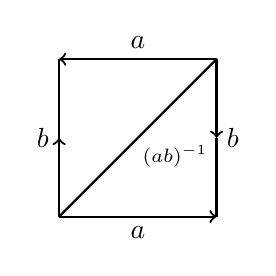
\begin{tikzpicture}[thick]
  \draw[->](0,0)--(0,1) node[anchor=east] {$b$};
  \draw[-](0,1)--(0,2);
  \draw[<-](0,2)--(1,2) node[anchor=south] {$a$};
  \draw[-](1,2)--(2,2);
  \draw[->](2,2)--(2,1)node[anchor=west] {$b$};
  \draw[-](2,1)--(2,0);
  \draw[<-](2,0)--(1,0) node[anchor=north] {$a$};
  \draw[-](1,0)--(0,0);
  \draw[-](0,0)--(2,2) node[yshift=-35, xshift=-15] {$\scriptstyle{(ab)^{-1}}$};
\end{tikzpicture}
\end{equation}
Here we have two $0$-chains $[a],[b]$ which are closed but $[(ab)^{-1}]=-[a]-[b]+\partial[\ldots]$. Therefore $H_{1}(T^{2})=\bbZ\oplus\bbZ$.

If we label the edges with the right group elements from $\bbA$ (so we put defects on the edges) and take a chain, we see that the closeness condition implies the group law
\begin{equation}
	\gamma=a[10]+b[20]+c[03]+\cdots
\end{equation}
then
\begin{equation}
	\left.\partial\gamma\right|_{[0]}=(a+b-c)[0]=0\implies a+b=c
\end{equation}
So a closed chain is in one-to-one correspondence with defects carrying group law. A chain $\gamma\in C_{d-p-1}(X,\bbA)$ is closed, then $\gamma$ corresponds to a $p$-form symmetry.

We also need to mod out for boundaries. Boundaries are nuclated whenever we have a loop in the network since they have to be closed by definition. Therefore, when we want to talk about defects, we not only require them to be closed but also mod out by nucleation which requires them to be in some homology group.

\subsection{Cohomology}
So we introduced the homology groups $\HH_j(X,\bbA)$ whose elements are closed chains which are not exact. We also found the physical correspondence of such objects: a $\gamma\in \HH_j$ is a newtork of $\bbA$-defects on a simplicial triangulation $\Delta(X)$ of some space-time manifold $X$\dots

We can now introduce the concept of \textit{co-chains}
\begin{defn}{Cochain}{}
	A co-chain $\nu$ is an element of 
	\begin{equation}
		C^j(X,\bbA)\equiv \mathrm{Hom}(C_j(X),\bbA)
	\end{equation}
	i.e. a map from chains to elements of an abelian group $\bbA$.
\end{defn}
As per the chains, cochains form an abelian group and we can define a differential
\begin{equation}
	\dd{}:C^j(X,\bbA)\rightarrow C^{j+1}(X,\bbA)
\end{equation}
which will act as expected: take $\nu\in C^j(X,\bbA)$, then
\begin{equation}
	\dd{\nu}(\gamma):=\nu(\partial\gamma)
\end{equation}
Clearly this is idempotent $\dd^2=0$. In components, by choosing a basis for $C_j(X)$, $\gamma=[i_0,\ldots, i_j]$ we have
\begin{equation}
	\nu\qty([i_0,\ldots, i_j])=\nu_{i_0\ldots i_j}\implies \dd{\nu}_{i_0\ldots i_j}=\sum_k (-1)^k \nu_{i_0\ldots i_{k-1}\;i_{k+1}\ldots i_j}
\end{equation}
Consider for example a $1$-cochain $\nu_{ij}$, we see that (using multiplicative notation)
\begin{equation}
	\dd{\nu}_{ijk}=\nu_{jk}\nu^{-1}_{ik}\nu_{ij}.
\end{equation}
Homology for cochains is called \textit{cohomology} and is given by the following co-chain complex
\begin{equation}
	\cdots\rightarrow C^j(X,\bbA)\xrightarrow{\dd}C^{j+1}(X,\bbA)\xrightarrow{\dd}C^{j+2}(X,\bbA)\xrightarrow{\dd}\cdots
\end{equation}
and
\begin{equation}
	\HH^j(X,\bbA)=\frac{\mathrm{Ker}(\dd_j)}{\mathrm{Im}(\dd_{j-1})}
\end{equation}
whose elements are flat connections which are not pure gauge.

On cohomology, we can define some natural operations
\begin{defn}{Cup-Product}{}
	Given a, possibly non-degenerate, pairing between abelian groups
	\begin{equation}
		(\;,\;):\bbA\times \bbB \rightarrow \bbD
	\end{equation}
	the \textit{cup product} is a product defined on co-cochains
	\begin{equation}
		\cup:C^j(X,\bbA)\times C^k(X,\bbB)\rightarrow C^{j+k}(X,\bbD)
	\end{equation}
	such that
	\begin{equation}
		(\mu \cup \nu)_{i_0,\ldots,i_{j+k}}\equiv (\mu_{i_0,\ldots, i_j},\nu_{i_j,\ldots, i_{j+k}})
	\end{equation}
\end{defn}
To have lift this to a good product in cohomology, we need it to be graded commutative. In general, given $A\in C^j, B\in C^k$
\begin{equation}
	\dd(A\cup B)=\dd{A}\cup \dd{B}+(-1)^j A\cup\dd{B}
\end{equation}
The product as defined on cochains is not, generally, graded commutative but the following
\begin{equation}
	A\cup B=(-1)^{jk}B\cup A+\dd{(A\cup_1 B)}+\dd{A}\cup_1 B+(-1)^j A\cup_1\dd{B}
\end{equation}
is graded commutative. The $\cup_1$ symbol is the Steenrod cup product and is another well defined product on cochains
\begin{equation}
	\cup_1:C^j\times C^k\rightarrow C^{j+k-1}
\end{equation}
This product is, on cohomology, graded commutative since $\dd{A}=0$, so we have defined a sensible product in cohomology.

Examples of reasonable parings are the following
\begin{itemize}
	\item Consider any abelian group $\bbA$ and $\bbB=\bbA^\vee\equiv \Hom(\bbA,\U(1))$ it's Pontrijagin dual. Elements of the Pontrijagin dual are just the characters of $\bbA$. Then the pairing is just given by
	\begin{equation}
		(a,\chi)=\chi(a)
	\end{equation}
	\item If both groups are $\bbZ_n$ then
	\begin{equation}
		(x,y)=xy\mod n
	\end{equation}
\end{itemize}
\subsection{Poincarè duality}
Poincarè duality over some space is an equivalence, if it exists, relating cohomology and homology on that space.\\
To do so, we need to introduce a method of adjoining chains and cochains. This is given by the cap product
\begin{defn}{Cap-product}{}
	Let $X$ be a topological space nd $\bbA$ some abelian group. The \textit{cap-product} is a bilinear map on homology and cohomology
	\begin{equation}
		\cap:H_j(X,\bbA)\times H^k(X,\bbA)\rightarrow H_{j-k}(X,\bbA),\qquad j>k
	\end{equation}
	defined by contracting a chain $\sigma\in C_j(X,\bbA)$ with a cochain $\mu\in C^k(X,\bbA)$ in the following manner
	\begin{equation}
		\sigma \cap \mu=\mu(\left.\sigma\right|_{[i_0,\ldots,i_k]})\left.\sigma\right|_{[i_k,\ldots,i_j]}
	\end{equation}
	Here the notation $\left.\sigma\right|_{[i_0,\ldots,i_k]}$ indicates the restriction of the simplicial map $\sigma$ to its face spanned by the vectors of the base.
\end{defn}
With this product at hand we can state the following theorem
\begin{thm}{Poincaré duality}{}
	If $X$ is a closed oriented $n$-mainifold with fundamental class $[X]\in H_n(X,\bbA)$, then the map 
	\begin{equation}
		\phi: H^k(X,\bbA)\rightarrow H_{n-k}(X,\bbA)
	\end{equation}
	defined by
	\begin{equation}
		\phi(\alpha)=[X]\cap \alpha
	\end{equation}
	is an isomorphism for all $k$.
\end{thm}
The relevance of this theorem in physics is that given a network of defects we have an associated gauge field and viceversa. So from $\gamma\in H_{d-p-1}(X,\bbA)$ we fin an $A\in H^{p+1}(X,\bbA)$. 

The idea of the proof is as follows: consider a triangulation $\Delta(X)$ and its dual $\overset{\vee}{\Delta}(X)$ constructed like a dual Bravais lattice in condensed matter
\begin{equation}
	\begin{tikzpicture}[thick]
		\path [fill=lightgray,draw] (0,-.5) to (2,0) to (1,2) to (0, -.5);
		\filldraw[black] (0,-.5) circle (2pt) node[]{};
		\filldraw[black] (2,0) circle (2pt) node[]{};
		\filldraw[black] (1,2) circle (2pt) node[]{};

		\path [fill=lightgray,draw] (5,-.5) to (7,0) to (6,2) to (5, -.5);
		\draw[-, red] (7,-.7)--(6,0.5);
		\draw[dashed, red] (6,0.5)--(5.59,0.99);
		\draw[-, red] (5.59,0.99)--(5,1.7);
	  	\filldraw[black] (5,-.5) circle (2pt) node[]{};
	  	\filldraw[black] (7,0) circle (2pt) node[]{};
	 	\filldraw[black] (6,2) circle (2pt) node[]{};
		

		\node at (1,-1.5) {$p$-simplex $\Delta^p\subset \Delta(X)$};
		\node at (6,-1.5) {$(d-p)$-simplex in red $\overset{\vee}{\Delta^p}\subset \Delta^{(d-p)}$};
  \end{tikzpicture}
\end{equation}
In general the dual triangulation is not a triangulation. 

So for example, in $2d$ a $1$-simplex and it's dual are the following\\
\begin{minipage}[c]{0.3\linewidth}
	\centering
		\begin{tikzpicture}[auto,baseline=(A)]
			%%%%%%%%%%%%%% nodes %%%%%%%%%%
			\node (A) at (0,0) {$0$};
			\node (B) at (3,0) {$1$};
			\node (C) at (1.5,3) {$2$};

			\filldraw[black] (0,0) circle (2pt) node[]{};
			
		\end{tikzpicture}
	\end{minipage}\hfill
	\begin{minipage}[c]{0.5\linewidth}
	\begin{equation}
		[01]\xlongrightarrow{P}[\overset{\vee}{0},\overset{\vee}{1}]=P([01])
	\end{equation}
\end{minipage}